\documentclass[a4j,dvipdfmx,titlepage]{jarticle}
\usepackage{multirow}
\usepackage{amsmath}
\usepackage[dvipdfmx]{graphicx}
\usepackage{slashbox}
\usepackage{bigstrut}
\usepackage{here}
\usepackage{cite}
\usepackage{listings,jlisting}
\usepackage{url}
\lstset{
  basicstyle={\ttfamily},
  identifierstyle={\small},
  commentstyle={\smallitshape},
  keywordstyle={\small\bfseries},
  ndkeywordstyle={\small},
  stringstyle={\small\ttfamily},
  frame={tb},
  breaklines=true,
  columns=[l]{fullflexible},
  numbers=left,
  xrightmargin=0zw,
  xleftmargin=3zw,
  numberstyle={\scriptsize},
  stepnumber=1,
  numbersep=1zw,
  lineskip=-0.5ex
}

\title{アルゴリズムとデータ構造}
\author{独立行政法人 国立高等専門学校機構長野工業高等専門学校
\\
3年 電子情報工学科
\\
渋谷圭亮
\\
}

\begin{document}
\maketitle
\section{目的}
カタラン定数$K$をC言語を用いた多倍長演算により、計算することを目的とする。
\section{原理}
まず、カタラン定数$K$は式1の通りに定義される。
\begin{eqnarray}
    \sum^{\infty}_{n=0}\frac{(-1)^{n}}{(2n+1)^2}=0.9159.....
\end{eqnarray}
今回は式1の計算を多倍長演算にて実装して、計算する。また、この式の演算により出力された値が正しいのかを確かめるために
同じカタラン定数を示す式2も実装する。\cite{catalan}\\
そして、これらで計算した値を比較することでカタラン定数を多倍長演算で正確に計算できたかを検証する。
\begin{eqnarray}
    K&=&\frac{1}{64}\sum^{\infty}_{n=1}\frac{(-1)^{n-1}2^{8n}(40n^2-24n+3)\{(2n)!\}^{3}(n!)^2}{n^3(2n-1)\{(4n)!\}^2}
\end{eqnarray}
\section{実験}
実際にC言語プログラムにて多倍長演算にて式1、式2らを実装する。
また今実験にてC言語プログラムを実行した環境を表\ref{a}に示す。
\begin{table}[H]
    \begin{center}
      \caption{実行環境}
      \begin{tabular}{c|c} 
       名称 & 型番 \\ \hline 
        CPU & AMD Ryzen 7 3700X\\
         M/B & Asrock X570 Taichi \\
         RAM &  Corsair CMW16GX4M2C3600C18\\
         GPU & GIGABYTE RTX 2070 Super AORUS\\
        OS & Ubuntu 18.04.5 LTS\\ 
        Compiler & gcc Version 7.5.0\\ 
      \end{tabular}
      \label{a}
\end{center}
\end{table}
今回の実験で作成したC言語プログラムをソースコード\ref{program}に示す。
\begin{lstlisting}[caption=今回作成したC言語プログラム,label=program]

#include <stdio.h>
#include <string.h>
#include <stdlib.h>
#include <limits.h>
#include <time.h>
#include <sys/timeb.h>

#define KETA 1000

typedef struct NUMBER
{
  int n[KETA];//各桁の値
  int sign;//符号
}Number;

int add(Number*, Number*, Number*);




//int sub(Number*, Number*, Number*);  //宣言

int setSign(Number* a, int s)
//多倍長変数aの符号を
//s=1なら正に,s=-1なら負に設定して0
//それ以外ならエラーとして-1
{
  if (s == 1)
  {
    a->sign = 1;
    return 0;
  }
  else if (s == -1)
  {
    a->sign = -1;
    return 0;
  }
  else
  {
    return -1;
  }
}

int getSign(Number* a)//aが0なら1を,負なら-1
{
  if (a->sign == 1)
  {
    return 1;
  }
  else
  {
    return -1;
  }
}

void clearByZero(Number* a)//多倍長変数の値を全部ゼロにし、+の符号をつける
{
  int i;

  for (i = 0; i < KETA; i++)  //すべての配列を0にセット
  {
    a->n[i] = 0;
  }

  setSign(a, 1);
}

void dispNumber(Number* a)//aを表示
{
  int i;

  if (getSign(a) == 1) 
  {
    printf("+");  //符号を先に出力
  }
  else 
  {
    printf("-");
  }

  for (i = KETA-1; i >= 0; i--) 
  {
    printf("%2d", a->n[i]);  //間隔をあける
  }
}

int zeroNumber(Number* a)
//多倍長変数の上位にある0を数える関数
//
//戻り値
//多倍長変数の上位にある0の数
{
  int zeroNumber = 0;
  int i;

  for (i = KETA - 1; i >= 0; i--)
  {
    if (a->n[i] == 0) //0があったのでzeronumberを足す
    {
      zeroNumber++;
    }
    else
    {
      break;
    }
  }

  return zeroNumber;  //返す
}



int isZero(Number* a)
//aがゼロか判別
//
//0・・・a==0
//-1・・・a!=0
{
  int i;

  if (getSign(a) == -1)  //マイナスなので
  {
    return -1;
  }

  for (i = 0; i < KETA; i++)
  {
    if (a->n[i] != 0) {
      return -1;
    }
  }

  return 0;  //終了
}

void copyNumber(Number* a, Number* b)//aをbにコピー
{
  int i;

  setSign(b,getSign(a));  //符号も忘れずに

  for (i = 0; i < KETA; i++) 
  {
    b->n[i] = a->n[i];
  }
}

void getAbs(Number* a, Number* b)//b=|a|
{
  copyNumber(a, b);
  setSign(b,1);
}

int mulBy10(Number* a, Number* b)
//aを10倍してbに返す
//
//戻り値
//0・・・正常終了
//-1・・・オーバーフロー
{
  int i;

  clearByZero(b);

  if (a->n[KETA - 1] != 0) 
  {
    return -1;
  }

  int zero = zeroNumber(a);

  for (i = 0; i < KETA - zero; i++) 
  {
    b->n[i + 1] = a->n[i];
  }

  b->n[0] = 0;
  setSign(b, getSign(a));

  return 0;
}

int mul10E(Number* a,int i){  //10^iした値を引数のところにまんま返す
  Number b;
  clearByZero(&b);

    while(1){
    mulBy10(a,&b);
    copyNumber(&b,a);
    if(i<=1){
      break;
    }
    i--;
  }

  
  return 0;
}



int divBy10(struct NUMBER *a , struct NUMBER *b){  //mulBy10の割り算バージョン
    int i;
  clearByZero(b);

    b->n[KETA-1] = 0;
    for(i=0;i<KETA-1;i++){
        b->n[i] = a->n[i+1];
    }
    return a->n[0];
}

int div10E(Number* a,int i){  //mul10Eの割り算バージョン
  Number b;
  clearByZero(&b);
  while(1){

    divBy10(a,&b);
    copyNumber(&b,a);
    if(i<=1){
      break;
    }
    i--;

  }

  
  return 0;
}


int setInt(Number* a, int x)
//多倍長変数aにint型変数xの値を設定する
//
//0・・・正常終了
//-1・・・xの値がaに設定しきれなかった
{
  int i;
  int Length = KETA;

  clearByZero(a);  //ひとまずキレイにする

  if (x < 0)  //負の値か区別
  {
    setSign(a, -1);

    for (i = 0; i < 10; i++)  //10進数であることに留意
    {
      if (x == 0)
      {
        return 0;
      }
      else if (Length == 0)
      {
        clearByZero(a);
        return -1;
      }
      a->n[i] = x % 10 * (-1);
      Length--;
      x = (x - x % 10) / 10;
    }
  }
  else
  {
    for (i = 0; i < 10; i++)
    {
      if (x == 0)
      {
        return 0;
      }
      else if (Length == 0)
      {
        clearByZero(a);
        return -1;
      }
      a->n[i] = x % 10;
      Length--;
      x = (x - x % 10) / 10;
    }
  }

  if (x == 0)
  {
    return 0;
  }
  else
  {
    clearByZero(a);
    return -1;
  }
}


int numComp(Number* a, Number* b)
//2つの多倍長変数a,bの大小を比較
//
//0・・・a==b
//1・・・a>b
//-1・・・a<b
{
  if (getSign(a) == 1 && getSign(b) == -1)
  {
    return 1;  //a>b
  }
  else if (getSign(a) == -1 && getSign(b) == 1)
  {
    return -1;  //a<b
  }
  else if (getSign(a) == 1 && getSign(b) == 1)   //同じ符号なので(+ +)
  {
    int aZero = zeroNumber(a);
    int bZero = zeroNumber(b);

    if (aZero > bZero)
    {
      return -1;  //上位の0の数を比較することで大きさを判別
    }
    else if (aZero < bZero)
    {
      return 1;
    }
    else   //判別できないので
    {
      int i;

      for (i = KETA - 1 - aZero; i >= 0; i--)  //1桁ずつ比較する
      {
        if (a->n[i] > b->n[i])
        {
          return 1;
        }
        else if (a->n[i] < b->n[i])
        {
          return -1;
        }
      }

      return 0;
    }
  }
  else
  {
    int aZero = zeroNumber(a);
    int bZero = zeroNumber(b);

    if (aZero > bZero)
    {
      return 1;
    }
    else if (aZero < bZero)
    {
      return -1;
    }
    else
    {
      int i;

      for (i = KETA - 1 - aZero; i >= 0; i--)
      {
        if (a->n[i] > b->n[i])
        {
          return -1;
        }
        else if (a->n[i] < b->n[i])
        {
          return 1;
        }
      }

      return 0;
    }
  }
}


int sub(Number* a, Number* b, Number* c)
//c <- a-b
//
//0・・・正常終了
//-1・・・オーバーフロー
{
  clearByZero(c);

  int i;
  int h = 0;
  int aSign = getSign(a);
  int bSign = getSign(b);

  if (aSign == 1 && bSign == 1)
  {
    if (isZero(a) == 0)
    {
      copyNumber(b, c);
      setSign(c, -1);
      return 0;
    }
    else if (isZero(b) == 0)
    {
      copyNumber(a, c);
      return 0;
    }


    if (numComp(a, b) == 1)
    {
      for (i = 0; i < KETA; i++)
      {
        if (a->n[i] < b->n[i] + h)
        {
          c->n[i] = 10 + a->n[i] - b->n[i] - h;
          h = 1;
        }
        else
        {
          c->n[i] = a->n[i] - b->n[i] - h;
          h = 0;
        }
      }
    }
    else if (numComp(a, b) == -1)
    {
      Number d;
      sub(b, a, &d);
      copyNumber(&d, c);
      setSign(c, -1);
    }

    return 0;
  }
  else if (aSign == 1 && bSign == -1)
  {
    Number d;
    getAbs(b, &d);
    int r = add(a, &d, c);
    return r;
  }
  else if (aSign == -1 && bSign == 1)
  {
    Number d;
    getAbs(a, &d);
    int r = add(&d, b, c);
    if (r == 0)
    {
      setSign(c, -1);
    }
    return r;
  }
  else
  {
    Number d, e;
    getAbs(a, &d);
    getAbs(b, &e);
    int r = sub(&e, &d, c);
    return r;
  }
}


int add(Number* a, Number* b, Number* c)
//c <- a+b
//
//0・・・正常終了
//-1・・・オーバーフロー
{
  int i, d;
  int e = 0;

  clearByZero(c);

  int aSign = getSign(a);
  int bSign = getSign(b);

  if (aSign == 1 && bSign == 1)
  {
    if (isZero(a) == 0)
    {
      copyNumber(b, c);
      return 0;
    }
    else if (isZero(b) == 0)
    {
      copyNumber(a, c);
      return 0;
    }


    for (i = 0; i < KETA; i++)
    {
      d = a->n[i] + b->n[i] + e;
      c->n[i] = d % 10;
      e = d / 10;
    }

    if (e != 0)
    {
      clearByZero(c);
      return -1;
    }

    return 0;
  }
  else if (aSign == 1 && bSign == -1)
  {
    Number d;
    getAbs(b, &d);
    int r = sub(a, &d, c);
    return r;
  }
  else if (aSign == -1 && bSign == 1)
  {
    Number d;
    getAbs(a, &d);
    int r = sub(b, &d, c);
    return r;
  }
  else
  {
    Number d, e;
    getAbs(a, &d);
    getAbs(b, &e);
    int r = add(&d, &e, c);
    if (r == 0)
    {
      setSign(c, -1);
    }
    return r;
  }
}

int increment(Number* a, Number* b)
//b <- a+1
{
  Number one;
  int r;

  setInt(&one, 1);
  r = add(a, &one, b);

  return r;
}

int inc(Number* a)
//a+1
{
  Number one, b;
  clearByZero(&b);

  int r;

  setInt(&one, 1);
  r = add(a, &one, &b);

  if (r == 0)
  {
    copyNumber(&b, a);
  }

  return r;
}

int decrement(Number* a, Number* b)
//b <- a-1
{
  Number one;
  int r;

  setInt(&one, 1);
  r = sub(a, &one, b);

  return r;
}
int dec(Number* a)
//a-1
{
  Number one, b;
  clearByZero(&b);
  int r;

  setInt(&one, 1);
  r = sub(a, &one, &b);

  if (r == 0)
  {
    copyNumber(&b, a);
  }

  return r;
}

int multiple(Number* a, Number* b, Number* c)
//c <- a*b
//
//0・・・正常終了
//-1・・・オーバーフロー
{
  int i, j, e, h, r;
  Number d,tmpC;

  int aSign = getSign(a);
  int bSign = getSign(b);
  int aZero = zeroNumber(a);
  int bZero = zeroNumber(b);
  
  clearByZero(c);

  if (isZero(a) == 0 || isZero(b) == 0)
  {
    return 0;
  }
  else if (aSign == 1 && bSign == 1)
  {
    clearByZero(&tmpC);

    for (i = 0; i < KETA - bZero + 1; i++)
    {
      h = 0;
      clearByZero(&d);

      for (j = 0; j < KETA - aZero + 1; j++)
      {
        e = a->n[j] * b->n[i] + h;
        if (i + j > KETA - 1 && e != 0)// a->n[] * b->[i] がオーバーフロー
        {
          clearByZero(c);
          return -1;
        }

        d.n[i + j] |= e % 10;
        h = (e - e % 10) / 10;
        if (h != 0 && i + j >= KETA - 1) //最上位の桁まで計算してもなお繰上りがある
        {
          clearByZero(c);
          return -1;
        }
      }

      r = add(&tmpC, &d, c);

      if (r == -1)//加算でオーバーフロー
      {
        return r;
      }

      copyNumber(c, &tmpC);
    }

    return 0;
  }
  else if (aSign == 1 && bSign == -1)
  {
    getAbs(b, &d);
    r = multiple(a, &d, c);
    if (r == 0)
    {
      setSign(c, -1);
    }
    return r;
  }
  else if (aSign == -1 && bSign == 1)
  {
    getAbs(a, &d);
    r = multiple(&d, b, c);
    if (r == 0)
    {
      setSign(c, -1);
    }
    return r;
  }
  else
  {
    Number f;
    getAbs(a, &d);
    getAbs(b, &f);
    r = multiple(&d, &f, c);
    return r;
  }
}

int divide(Number* a, Number* b, Number* c, Number* d)
//
//c <- 商
//d <- あまり
//0...正常終了
//-1...割る数が0
{
  Number n, m;

  clearByZero(c);
  clearByZero(d);

  if (isZero(b) == 0)
  {
    return -1;
  }

  int aSign = getSign(a);
  int bSign = getSign(b);

  if (aSign == 1 && bSign == 1)
  {
    copyNumber(a, &n);

    while (1)
    {
      if (numComp(&n, b) == -1)
      {
        copyNumber(&n, d);
        return 0;
      }
      else
      {
        increment(c, &m);
        copyNumber(&m, c);
        sub(&n, b, &m);
        copyNumber(&m, &n);
      }
    }
  }
  else if (aSign == 1 && bSign == -1)
  {
    Number p;
    getAbs(b, &p);
    divide(a, &p, c, d);
    setSign(c, -1);
  }
  else if (aSign == -1 && bSign == 1)
  {
    Number p;
    getAbs(a, &p);
    divide(&p, b, c, d);
    setSign(c, -1);
    setSign(d, -1);
  }
  else
  {
    Number p, q;
    getAbs(a, &p);
    getAbs(b, &q);
    divide(&p, &q, c, d);
    setSign(d, -1);
  }
}

int power(Number* a, Number* b, Number* c) 


//
//c <- a^b
//0...正常終了
//-1...オーバーフローまたはアンダーフロー
//-1...b < 0
{
  clearByZero(c);
  Number one,two,d,gm,tmp,tmp1;
  int r;

  int aZero = isZero(a);
  int bZero = isZero(b);

  if (numComp(b, c) == -1)
  {
    return -2;
  }

  increment(c, &one);

  if (bZero == 0)
  {
    setInt(c, 1);
    return 0;
  }
  if (aZero == 0)
  {
    clearByZero(c);
    return 0;
  }
  
  if (numComp(a, &one) == 0)
  {
    setInt(c, 1);
    return 0;
  }
  if (numComp(b, &one) == 0)
  {
    copyNumber(a, c);
    return 0;
  }

  increment(&one, &two);

  if(b->n[0] % 2 == 0)
  {
    r = multiple(a, a, &tmp);
    if (r == -1)
    {
      clearByZero(c);
      return -1;
    }

    divide(b, &two, &d, &gm);
    r = power(&tmp, &d, c);
    if (r == -1)
    {
      clearByZero(c);
      return -1;
    }

    return 0;
  }
  else
  {
    decrement(b, &tmp1);
    r = power(a, &tmp1, &tmp);
    if (r == -1)
    {
      clearByZero(c);
      return -1;
    }

    r = multiple(a, &tmp, c);
    if (r == -1)
    {
      clearByZero(c);
      return -1;
    }

    return 0;
  }
}


int inverseNumber(Number* a,Number* b,int p){ //aの逆数をNumber* b に返す  pは精度 この逆数ルーチンは2次収束
  Number eps,x,y,g,x1,pow1,pow2,pow3,tei1,tei2,tei0,h,j,a1;
  int i,c1,c0,c2;
  int n = KETA - zeroNumber(a); //n = N+1 =log_10(a)
      //ずらす分の10^p
    c2=1;

  c0=isZero(a); //最初にaについて判定して実行できるか確かめる
  if(c0==0){
    printf("異常終了");
    return -1;
  }
  c0=getSign(a);
  if(c0==-1){
    setSign(a,1); //いったん+にセットする
    c2=-1; //あとで-の符号をつけるために
  }

  //初期値セット
  setInt(&eps,1);
  //mul10E(&eps,9); //機械イプシロンのセット ε=1

  setInt(&tei2,2);
  copyNumber(&tei2,&x);

  c1=p-n-1;  //ずらす

  mul10E(&x,c1);  //x=2.0*10^{p-n-1}
  setInt(&tei0,2);
  mul10E(&tei0,p);  //x=y*(2.0-a*y)の2.0も10^p倍する


  while(1){
    copyNumber(&x,&y);  //1つ前のx

    multiple(a,&y,&tei2);  //te2=a*y

    sub(&tei0,&tei2,&h);  //2.0-a*y=h
    
    multiple(&y,&h,&x); //x=y*(2.0-a*y)

    div10E(&x,p);   //ずれてんのでその分直す

    sub(&x,&y,&j);  //j=x-y

    getAbs(&j,&g);   //直す	

    if(numComp(&g,&eps)==-1||numComp(&g,&eps)==0){
      break; //g<epsと比較することで十分に正確な値を求め切ったかを確認
    }
  }

  if(c2<0){
    setSign(&x,(int)-1); //-にセットする
  }

  copyNumber(&x,b); //逆数を返すところにx(答え)を入れる

  return 0; //正常終
}

int ultimatedivide(Number* a, Number* b, Number* c)
//NewtonRapson法を応用した除算
//c <- a/b
//0...正常終了
//-1...割る数が0
{
  Number m,d,e;

  int n=KETA-zeroNumber(a)+5;  //精度

  clearByZero(c);
  clearByZero(&e);
  
  if (isZero(b) == 0)
  {
    return -1;
  }

  int aSign = getSign(a);  //被除数の符号取得
  int bSign = getSign(b);  //除数の符号取得

  if (aSign == 1 && bSign == 1) //+の時
  {
    inverseNumber(b,&d,n);  //除数の逆数をとる
    multiple(a,&d,&e);   //Q=NX(被除数×除数の逆数)
    div10E(&e,n);  //ずらす
    copyNumber(&e,c);   //答えをcに返す

      
    }
  else if (aSign == 1 && bSign == -1)  //被除数(+) 除数(-)
  {
    Number p;
    getAbs(b, &p);
    ultimatedivide(a, &p, c);
    setSign(c, -1);
  }
  else if (aSign == -1 && bSign == 1)  //被除数(-) 除数(+)
  {
    Number p;
    getAbs(a, &p);
    ultimatedivide(&p, b, c);
    setSign(c, -1);
  }
  else  //両方とも(-)
  {
    Number p, q;
    getAbs(a, &p);
    getAbs(b, &q);
    ultimatedivide(&p, &q, c);
  }
}

Number kaijo(Number* a){  //階乗を行う

    Number a1,b,one,i;

    setInt(&a1,1);
    setInt(&i,1);

    while(1){
        multiple(&a1,&i,&b);  //b=a*i
        copyNumber(&b,&a1);   //a==b    a*=i
        inc(&i);
        if(numComp(&i,a)==1){  //i>aなのでやめようね
            break;
        }
    }
  copyNumber(&a1,a);  //引数のやつにも答えを入れる
    return a1;  //答えを返すお
}

Number kensan2(int keta){   
    Number Keta,bunbo,bunshi,one,eps,two,forty,twe4,three,four,eight,six4,n,n8,c1,c2,c3,c0,c4,c5,h,h1,value,twon,tmp,before;
  int flag=0;
  keta+=1;

  clearByZero(&bunbo);  
  clearByZero(&bunshi);
  clearByZero(&value);
  clearByZero(&before);
  setInt(&one,1);
  setInt(&Keta,1);
  setInt(&eps,1);
  setInt(&two,2);
  setInt(&forty,40);
  setInt(&twe4,24);
  setInt(&three,3);
  setInt(&four,4);
  setInt(&eight,8);
  setInt(&six4,64);
  copyNumber(&one,&n);    //n=1


  mul10E(&Keta,keta);  //Keta=10^{keta}


  while(1){

    copyNumber(&value,&before);

    multiple(&eight,&n,&n8);  //n8=8*n

    power(&two,&n8,&c1); //c1=2^(8*n)  

    power(&n,&two,&n8); //n8=n^2

      multiple(&forty,&n8,&c0);   //c0=40*n^2
    multiple(&twe4,&n,&c2);  //c2=24*n
    sub(&c0,&c2,&c3);  //c0-c2=c3
    add(&c3,&three,&c2);  //c2=c3+3   →40*n^2-24*n+3 =c2

    multiple(&two,&n,&n8);  //n8=2*n
    copyNumber(&n8,&twon);  //twon=2*n
    
    kaijo(&n8);  //n8=(2*n)!
    power(&n8,&three,&c3);  //c3=((2*n!))^3

      copyNumber(&n,&c4);  //c4=n  
    kaijo(&c4);  //c4=n!
    power(&c4,&two,&c0);  //c0=(n!)^2


    multiple(&c1,&c2,&c4);  //c4=c1*c2
    multiple(&c3,&c0,&c5);  //c5=c0*c3

    //c4*c5=分子


    multiple(&c4,&c5,&bunshi);

    multiple(&bunshi,&Keta,&c4);  //正確に計算
    copyNumber(&c4,&bunshi);
    //ここまでで分子

    power(&n,&three,&c0);  //c0=n^3
    sub(&twon,&one,&c1);  //c1=2*n-1
    multiple(&two,&twon,&c3);   //c3=(2*n)*2=4*n
    kaijo(&c3); //(4*n)!
        power(&c3,&two,&c4);   //c4=(4*n!)^2

    multiple(&c0,&c1,&c5);   //c5=c0*c1=(n^3)*(2*n-1)
    multiple(&c5,&c4,&bunbo);   //bunbo=c5*c4=c5*((4*n!)^2)
    multiple(&six4,&bunbo,&c5);
    copyNumber(&c5,&bunbo);  

    //ここまでで分母求めた  64*n^3*(2*n-1)*[(4*n)!]^2

    ultimatedivide(&bunshi,&bunbo,&h);  //h=Σのところ

    if (isZero(&h)==0)  //たばいちょうで計算できる桁数超えそうになったらおしまい
    {
      
      
      break;
    }



    if(n.n[0]%2==0){  //+もしくは-かをつける

      sub(&value, &h, &h1);  //h1=value-h
      copyNumber(&h1, &value);  //value-=h

    }
    else{
      add(&value, &h, &h1);  //h1=value+h
      copyNumber(&h1, &value);  //value+=h
    }


    inc(&n);
    flag++;


  }

  printf("%d回ループ\n",flag);

  div10E(&value,1);

  return value;
}

Number catalan2(int keta) //カタラン定数を定義により求める
{
  Number value, a, two, loop, tmp, tmp1, tmp2, Keta,eps;
  int i=0;
  keta+=2;

  setInt(&two, 2);
  clearByZero(&loop);
  setInt(&Keta,1);
  clearByZero(&value);
  clearByZero(&tmp);
  clearByZero(&tmp2);
  setInt(&eps,1);


  mul10E(&Keta,keta);
  
  
  while (1)
  {
    multiple(&two, &loop, &tmp);  //tmp=2*n
    inc(&tmp);  //インクリメント  2*n+1
    power(&tmp, &two, &tmp1);  //(2*n+1)^2=tmp1

    if (numComp(&Keta,&tmp1)==-1)  //たばいちょうで計算できる桁数超えそうになったらおしまい
    {
      break;
    }




    ultimatedivide(&Keta, &tmp1, &a);  //a<=Keta/tmp1   
    if (loop.n[0] % 2 == 0)  //奇数偶数で計算パターンを変更
    {
      add(&value, &a, &tmp2);  //tmp2=value+a
      copyNumber(&tmp2, &value);  //value=tmp2  すなわちvalue+=a
    }
    else
    {
      sub(&value, &a, &tmp2);  //tmp2=value-a
      copyNumber(&tmp2, &value);  //value-=a
    }
    inc(&loop);  //loop++(n++)
    i++;
    
  }
  printf("%d回ループ\n",i);
  div10E(&value,2);  
  return value;
}

int main(){

  clock_t start,end;
  start=clock();
  int a=10;
  Number C,B,D;
  clearByZero(&C); 
  C=kensan2(a);
  dispNumber(&C);
  printf("\n"); 
  clearByZero(&D);
  D=catalan2(a);
  dispNumber(&D);
  if(numComp(&C,&D)==0){
    printf("\n");
    printf("定義式で計算した値と検算用の式で計算した値は一致した。");
  }  

  end = clock();
  printf("\n");
  printf("%.6f[s]\n",(double)(end-start)/CLOCKS_PER_SEC);
  

  
}  
\end{lstlisting}
カタラン定数の計算で使用する式1は非常に収束が遅いため、もとめる桁数は10桁とする。
収束が遅いことにより、式1のとおり計算を行うcatalan2関数の計算量は桁数が増えるにつれて膨大になっていく。
その様子を図\ref{teigi}に示す。 縦軸のloop(回)とはwhile文が回る回数を示す。
\begin{figure}[H]
  \begin{center}
    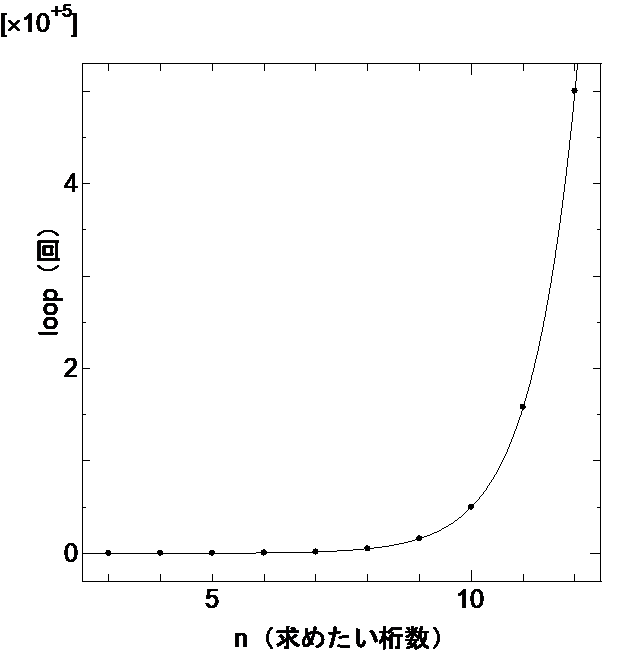
\includegraphics[height=8.0cm]{teigi.png}
    \caption{catalan2関数の計算量}
    \label{teigi}
  \end{center}
\end{figure}
今回作成したプログラムについておおまかに説明する。
kensan2関数では引数(int型)分の桁数ほどカタラン定数を式2の通り計算する。
また、catalan2関数では引数(int型)分の桁数ほどカタラン定数を式1の通り計算する。
これらの計算に必要な級数表現はwhile文を用いて再現し、四則演算または階乗、累乗はそれぞれの処理を行う関数を作成することで
可能にした。そして、これらの関数は精度向上のために、引数分の桁数より少し多い桁数で計算をしているため、whileのループを抜けたあとに計算値を返す前に余計に多い桁数だけ10で割っている。
main関数では指定した桁数だけcatalan2関数もしくはkensan2関数で計算させた後にnumcomp関数という引数となる値2つを比較する関数に渡すことによって、式1によって計算したカタラン定数の検算を行っている。
%まだ書きかけ

\section{実行結果}
実行結果をソースコード\ref{kekka}に示す。
\begin{lstlisting}[caption=実行結果,label=kekka]
  18回ループ
  + 0 0 0 0 0 0 0 0 0 0 0 0 0 0 0 0 0 0 0 0 0 0 0 0 0 0 0 0 0 0 0 0 0 0 0 0 0 0 0 0 0 0 0 0 0 0 0 0 0 0 0 0 0 0 0 0 0 0 0 0 0 0 0 0 0 0 0 0 0 0 0 0 0 0 0 0 0 0 0 0 0 0 0 0 0 0 0 0 0 0 0 0 0 0 0 0 0 0 0 0 0 0 0 0 0 0 0 0 0 0 0 0 0 0 0 0 0 0 0 0 0 0 0 0 0 0 0 0 0 0 0 0 0 0 0 0 0 0 0 0 0 0 0 0 0 0 0 0 0 0 0 0 0 0 0 0 0 0 0 0 0 0 0 0 0 0 0 0 0 0 0 0 0 0 0 0 0 0 0 0 0 0 0 0 0 0 0 0 0 0 0 0 0 0 0 0 0 0 0 0 0 0 0 0 0 0 0 0 0 0 0 0 0 0 0 0 0 0 0 0 0 0 0 0 0 0 0 0 0 0 0 0 0 0 0 0 
  0 0 0 0 0 0 0 0 0 0 0 0 0 0 0 0 0 0 0 0 0 0 0 0 0 0 0 0 0 0 0 0 0 0 0 0 0 0 0 0 0 0 0 0 0 0 0 0 0 0 0 0 0 0 0 0 0 0 0 0 0 0 0 0 0 0 0 0 0 0 0 0 0 0 0 0 0 0 0 0 0 0 0 0 0 0 0 0 0 0 0 0 0 0 0 0 0 0 0 0 0 0 0 0 0 0 0 0 0 0 0 0 0 0 0 0 0 0 0 0 0 0 0 0 0 0 0 0 0 0 0 0 0 0 0 0 0 0 0 0 0 0 0 0 0 0 0 0 0 0 0 0 0 0 0 0 0 0 0 0 0 0 0 0 0 0 0 0 0 0 0 0 0 0 0 0 0 0 0 0 0 0 0 0 0 0 0 0 0 0 0 0 0 0 0 0 0 0 0 0 0 0 0 0 0 0 0 0 0 0 0 0 0 0 0 0 0 0 0 0 0 0 0 0 0 0 0 0 0 0 0 0 0 0 0 0 0 
  0 0 0 0 0 0 0 0 0 0 0 0 0 0 0 0 0 0 0 0 0 0 0 0 0 0 0 0 0 0 0 0 0 0 0 0 0 0 0 0 0 0 0 0 0 0 0 0 0 0 0 0 0 0 0 0 0 0 0 0 0 0 0 0 0 0 0 0 0 0 0 0 0 0 0 0 0 0 0 0 0 0 0 0 0 0 0 0 0 0 0 0 0 0 0 0 0 0 0 0 0 0 0 0 0 0 0 0 0 0 0 0 0 0 0 0 0 0 0 0 0 0 0 0 0 0 0 0 0 0 0 0 0 0 0 0 0 0 0 0 0 0 0 0 0 0 0 0 0 0 0 0 0 0 0 0 0 0 0 0 0 0 0 0 0 0 0 0 0 0 0 0 0 0 0 0 0 0 0 0 0 0 0 0 0 0 0 0 0 0 0 0 0 0 0 0 0 0 0 0 0 0 0 0 0 0 0 0 0 0 0 0 0 0 0 0 0 0 0 0 0 0 0 0 0 0 0 0 0 0 0 0 0 0 0 0 0 
  0 0 0 0 0 0 0 0 0 0 0 0 0 0 0 0 0 0 0 0 0 0 0 0 0 0 0 0 0 0 0 0 0 0 0 0 0 0 0 0 0 0 0 0 0 0 0 0 0 0 0 0 0 0 0 0 0 0 0 0 0 0 0 0 0 0 0 0 0 0 0 0 0 0 0 0 0 0 0 0 0 0 0 0 0 0 0 0 0 0 0 0 0 0 0 0 0 0 0 0 0 0 0 0 0 0 0 0 0 0 0 0 0 0 0 0 0 0 0 0 0 0 0 0 0 0 0 0 0 0 0 0 0 0 0 0 0 0 0 0 0 0 0 0 0 0 0 0 0 0 0 0 0 0 0 0 0 0 0 0 0 0 0 0 0 0 0 0 0 0 0 0 0 0 0 0 0 0 0 0 0 0 0 0 0 0 0 0 0 0 0 0 0 0 0 0 0 0 0 0 0 0 0 0 0 0 0 0 0 0 0 0 0 0 0 0 0 0 0 0 0 0 0 0 0 0 0 0 0 0 0 0 0 0 0 0 0 
  0 0 0 0 0 0 0 0 0 0 0 0 0 0 0 0 0 0 0 0 0 0 0 0 0 0 0 0 0 0 0 0 0 0 0 0 0 0 0 0 0 0 0 9 1 5 9 6 5 5 9 4 1
  500000回ループ
  + 0 0 0 0 0 0 0 0 0 0 0 0 0 0 0 0 0 0 0 0 0 0 0 0 0 0 0 0 0 0 0 0 0 0 0 0 0 0 0 0 0 0 0 0 0 0 0 0 0 0 0 0 0 0 0 0 0 0 0 0 0 0 0 0 0 0 0 0 0 0 0 0 0 0 0 0 0 0 0 0 0 0 0 0 0 0 0 0 0 0 0 0 0 0 0 0 0 0 0 0 0 0 0 0 0 0 0 0 0 0 0 0 0 0 0 0 0 0 0 0 0 0 0 0 0 0 0 0 0 0 0 0 0 0 0 0 0 0 0 0 0 0 0 0 0 0 0 0 0 0 0 0 0 0 0 0 0 0 0 0 0 0 0 0 0 0 0 0 0 0 0 0 0 0 0 0 0 0 0 0 0 0 0 0 0 0 0 0 0 0 0 0 0 0 0 0 0 0 0 0 0 0 0 0 0 0 0 0 0 0 0 0 0 0 0 0 0 0 0 0 0 0 0 0 0 0 0 0 0 0 0 0 0 0 0 0 
  0 0 0 0 0 0 0 0 0 0 0 0 0 0 0 0 0 0 0 0 0 0 0 0 0 0 0 0 0 0 0 0 0 0 0 0 0 0 0 0 0 0 0 0 0 0 0 0 0 0 0 0 0 0 0 0 0 0 0 0 0 0 0 0 0 0 0 0 0 0 0 0 0 0 0 0 0 0 0 0 0 0 0 0 0 0 0 0 0 0 0 0 0 0 0 0 0 0 0 0 0 0 0 0 0 0 0 0 0 0 0 0 0 0 0 0 0 0 0 0 0 0 0 0 0 0 0 0 0 0 0 0 0 0 0 0 0 0 0 0 0 0 0 0 0 0 0 0 0 0 0 0 0 0 0 0 0 0 0 0 0 0 0 0 0 0 0 0 0 0 0 0 0 0 0 0 0 0 0 0 0 0 0 0 0 0 0 0 0 0 0 0 0 0 0 0 0 0 0 0 0 0 0 0 0 0 0 0 0 0 0 0 0 0 0 0 0 0 0 0 0 0 0 0 0 0 0 0 0 0 0 0 0 0 0 0 0 
  0 0 0 0 0 0 0 0 0 0 0 0 0 0 0 0 0 0 0 0 0 0 0 0 0 0 0 0 0 0 0 0 0 0 0 0 0 0 0 0 0 0 0 0 0 0 0 0 0 0 0 0 0 0 0 0 0 0 0 0 0 0 0 0 0 0 0 0 0 0 0 0 0 0 0 0 0 0 0 0 0 0 0 0 0 0 0 0 0 0 0 0 0 0 0 0 0 0 0 0 0 0 0 0 0 0 0 0 0 0 0 0 0 0 0 0 0 0 0 0 0 0 0 0 0 0 0 0 0 0 0 0 0 0 0 0 0 0 0 0 0 0 0 0 0 0 0 0 0 0 0 0 0 0 0 0 0 0 0 0 0 0 0 0 0 0 0 0 0 0 0 0 0 0 0 0 0 0 0 0 0 0 0 0 0 0 0 0 0 0 0 0 0 0 0 0 0 0 0 0 0 0 0 0 0 0 0 0 0 0 0 0 0 0 0 0 0 0 0 0 0 0 0 0 0 0 0 0 0 0 0 0 0 0 0 0 0 
  0 0 0 0 0 0 0 0 0 0 0 0 0 0 0 0 0 0 0 0 0 0 0 0 0 0 0 0 0 0 0 0 0 0 0 0 0 0 0 0 0 0 0 0 0 0 0 0 0 0 0 0 0 0 0 0 0 0 0 0 0 0 0 0 0 0 0 0 0 0 0 0 0 0 0 0 0 0 0 0 0 0 0 0 0 0 0 0 0 0 0 0 0 0 0 0 0 0 0 0 0 0 0 0 0 0 0 0 0 0 0 0 0 0 0 0 0 0 0 0 0 0 0 0 0 0 0 0 0 0 0 0 0 0 0 0 0 0 0 0 0 0 0 0 0 0 0 0 0 0 0 0 0 0 0 0 0 0 0 0 0 0 0 0 0 0 0 0 0 0 0 0 0 0 0 0 0 0 0 0 0 0 0 0 0 0 0 0 0 0 0 0 0 0 0 0 0 0 0 0 0 0 0 0 0 0 0 0 0 0 0 0 0 0 0 0 0 0 0 0 0 0 0 0 0 0 0 0 0 0 0 0 0 0 0 0 0 
  0 0 0 0 0 0 0 0 0 0 0 0 0 0 0 0 0 0 0 0 0 0 0 0 0 0 0 0 0 0 0 0 0 0 0 0 0 0 0 0 0 0 0 9 1 5 9 6 5 5 9 4 1
  定義式で計算した値と検算用の式で計算した値は一致した。
  1333.416000[s]
\end{lstlisting}
作成したプログラムと照らし合わせると、CとDの値が完全に一致している時のみ表示される文字が出力されているといえるため、式1のとおり計算したカタラン定数の値は正しいといえる。
\begin{thebibliography}{99}
  \bibitem{catalan} Catalan's Constant \url{https://mathworld.wolfram.com/CatalansConstant.html}
\end{thebibliography}






\end{document}